The application is written in Java. The main reason for this is its cross-platform compatibility. Students can run it on any department-supported Operating System: Windows, Linux or Mac OS. The application has four main components:

A \emph{Parser} validates the input assembler file's syntax, informing the user of any errors. It builds an \emph{Abstract Syntax Tree} (AST) of sorts, which is passed to the Assembler.

An \emph{Assembler} translates the MIPS instructions in this AST to machine code; the machine code is stored in the \emph{Memory Manager}.

Next, a virtual \emph{Processor} is activated and interprets the machine code. It simulates the actions, recording input or displaying output where necessary.

The final component is the \emph{User Interface}. There are two versions:
\begin{itemize}
\item a \emph{text only} interface which accepts input from and prints output to a command line (be it the UNIX console, DOS, ...).
\item a \emph{Graphical User Interface} (GUI).
\end{itemize}

Both have a central \emph{Controller} class which communicates with the three components above. In the case of the \emph{text only} version, this controller class is the \emph{YAMSConsole}. It handles command line input and deals with the overall flow of the program. The equivalent for the GUI will be discussed in Chapter 3.

\section{Lexer and Parser}

The Lexer and Parser (hereafter simply referred to as the Parser), has the task of reading in assembler source files (\emph{*.asm} files) and building the AST. This AST is, in fact, linear due to the nature of assembler programs and has thus been modelled as a {\tt LineList}. This class is described in figure \ref{figLineList}.

\begin{figure}[htbp]
\begin{center}
\includegraphics[width=7cm]{linelist.eps}
\end{center}
\caption{LineList}
\label{figLineList}
\end{figure}

A {\tt LineList} object contains a list of {\tt Line} objects. Each {\tt Line} object contains either a {\tt Label}, an {\tt Instruction}, or both. 

Instructions are either R-type, I-type or J-type and, depending on their type, contain one, two or three operands. Operands can be one of six types, as illustrated in figure \ref{figOperands}.

Alternatively, Instrucions can be of type {\tt Directive} followed by a list of operands (possibly empty).

\begin{figure}[htbp]
\begin{center}
\includegraphics[height=7cm]{operands.eps}
\end{center}
\caption{Operands}
\label{figOperands}
\end{figure}

The {\tt Lexer} tokenizes the input from an assembler file and control is passed to the {\tt Parser}. The {\tt Parser} attempts to translate a line of tokens into an object of type {\tt Instruction}. Parse errors are immediately reported to the user and must be corrected before continuing to the next stage.

\section{Assembler}

When the Assembler object is created, the first thing is does is create an {\tt AssemblerXMLHandler} which is used to access the XML file where all of the MIPS Instructions' behaviour is specified. The {\tt Assembler} builds the {\tt InstructionTable}, a lookup table for instructions and their machine code representation.

The {\tt LineList} object returned by the Parser is passed to the {\tt Assembler} which iterates through it line-by-line.

If the line contains a label, a reference to it is stored in the {\tt SymbolTable}.

If the line contains an instruction, it is assembled to machine code using the template given by the {\tt InstructionTable}. If an instruction contains a label, this is looked up in the {\tt SymbolTable}. Sometimes, however, a label may be encountered before being defined in the assembler file. In such a case, the assembler adds a note to the {\tt ToBeDoneList} and continues. After completing one pass of the list, all labels should have been defined. At this point the assembler verifies that all symbols in the {\tt ToBeDoneList} do indeed refer to an entry in the {\tt SymbolTable}.


\section{Processor}

The {\tt Processor} is created in the controller (either {\tt YAMSConsole} or {\tt YAMSGui}. The classes' main job is to create and co-ordinate activity between the Processor's constituent components. These include: 
\begin{itemize}
\item Cycle Manager
\item Register Manager
\item Memory Manager
\item System Call Handler
\item Instruction Handler
\item Instruction Decoder
\end{itemize}

The Cycle Manager, whilst running, executes machine code instructions which have been stored in the Memory Manager. It looks up the current instruction using the Program Counter register, with the aid of the Register Manager, and tries to execute it using the Instruction Decoder.

The Instruction Decoder converts the instruction to a string of 32 bits in order to make it easier to manipulate. It then attempts to identify which instruction it is and calls the corresponding code from the Instruction Handler or, in the case of a system call, the System Call Handler.

The Instruction Handler and the System Call Handler were automatically generated form the XML file, so that the instruction set can be extended without changing any of the source code files. The XML file includes a small amount of Java code for each instruction describing what it does and, of course, it has access to the Register Manager and Memory Manager.

The Register Manager and Memory Manager provide access to the Registers and Memory respectively. In order to make the simulation reflect reality as far as possible, the Memory Manager only has public methods, for reading from and writing to memory. Similarly, the Register Manager can only read from and write to registers. We could have included more complicated access methods but felt that this was giving too much responsibility to an otherwise simple part of the processor.
